\graphicspath{{chapters/17/images}}
\chapter{Monte Carlo methods}

\section{Introduction}
Monte Carlo methods are based on games of chance.
Trying to evaluate the following integral:

$$I = \int_0^1dx\int_0^{\sqrt{1-x^2}}dy = \frac{\pi}{4}$$

	\subsection{Central limit theorem}
	Let $f$ be an arbitrary function such that:

	$$f(x)\ge 0\qquad \int f(x)dx = 1$$

	And:

	$$I = \int dx\phi(x)f(x)\equiv\langle\phi\rangle_f$$

	Let $x_1, \dots, x_M$ n-dimensional vectors sampled from $f(x)$.
	Then by the central limit theorem:

	$$\tilde{I}_M = \frac{1}{M}\sum\limits_{i=1}^M\phi(x_i)\qquad \lim\limits_{M\rightarrow\infty}\tilde{I}_M = I$$

	$$\int dx\phi(x)f(x) = \frac{1}{M}\sum\limits_{i=1}^M\phi(x_i)\pm\frac{1}{\sqrt{M}}\bigl[\langle\phi^2\rangle_f-\langle\phi\rangle_f^2\bigr]^{\frac{1}{2}}$$

	\subsection{Sampling distributions}
	One dimensional distribution function:

	$$\int_a^bf(x)dx = 1\qquad f(x)\ge 0$$

	$$P(X) = \int_a^X f(x)dx\qquad X\in[a,b]$$

	$P(X)$ is the probability that any chosen $x$ from the distribution $f(x)$ lies in $[a, X]$.
	$P(X)$ is a monotonically increasing function of $X$:

	$$f(X) = Fraec{dP}{dX}$$

	Variable transformation $x\rightarrow y$ with $y = g(x)$ non decreasing function of $x$:

	$$X\ge x \Rightarrow g(X) \ge g(x)$$

	$\tilde{P}(Y=g(X))$ is the probability that $g(X)\ge g(x)$, the probability that $X\ge x$.

	$$\tilde{P}(Y) = P(X)$$

	$$w(r) = \begin{cases}1 &0\le r\le 1\\0 &otherwise\end{cases}\qquad W(\xi) = \int_0^\xi w(r)ds = \begin{cases}0 & \xi<0\\\xi & 0\le\xi\le1\\1 &otherwise\end{cases}$$

	$W(`x) = \xi$ is the probability that $r$ chosen randomly lies in $[0, \xi]$.
	$r = g(x)$ with $g(x)$ a non decreasing function: solve $P(X) = \xi$.

		\subsubsection{An example}

		$$f(x) = ce^{-cx}\qquad x\in[0, +\infty[$$

		$$P(X) = \int_0^Xce^{-cx}dx = 1- e^{-cX} = \xi\Rightarrow X = -\frac{1}{C}\ln(1-\xi)$$

		The same procedure can be generalized to more than one random variable easily when $f(x)$ is separable into a product of $n$ single-variable distributions.

	\subsection{Importance sampling}

	$$I = \int dx\phi(x)f(x) = \int dx\biggl[\frac{\phi(x)f(x)}{h(x)}\biggr]h(x) = \int dx\psi(x)h(x)$$

	$$I = \int dx\psi(x)h(x) = \frac{1}{M}\sum\limits_{i=1}^M\psi(x_i)\pm\frac{1}{\sqrt{M}}[\langle\psi^2\rangle_h-\langle\psi\rangle_h^2]^{\frac{1}{2}}$$

	This is done because $h(x)$ might be easier to sample or it might behave better than $f(x)$.
	The optimal choice for $h(x)$:

	$$\sigma^2[h] = \int dx\psi^2(x)h(x) - \biggl[\int dx\psi(x)h(x)\biggr]^2 = \int dx\frac{\phi^2(x)f^2(x)}{h(x)}-\biggl[\int dx\phi(x)f(x)\biggr]^2$$

	Minimize $\sigma^2[h]$ with the constraint $\int dx h(x) = 1$.
	Lagrange multiplier: $F[h] = \sigma^2[h]-\lambda\int dxh(x)$.
	Functional derivative: $\frac{\delta F[h]}{\delta h(x)} = 0$ with $\delta F[h] = F[h+\delta h]-F[h]$.
	Now:

	\begin{align*}
		\delta F[h] &= \int dx\biggl[\frac{\phi^2(x)f^2(x)}{h(x) + \delta h(x)} - \frac{\phi^2(x)f^2(x)}{h(x)}\biggr]-\lambda\delta h(x)=\\
								&=-\frac{\phi^2(x)f^2(x)}{h^2(x)}\delta h(x)-\lambda\delta h(x)
	\end{align*}

	$$\frac{\delta F[h]}{\delta h(x)} = 0\Rightarrow\frac{\phi^2(x)f^2(x)}{h^2(x)}+\lambda = 0\Rightarrow h(x) = \frac{1}{\sqrt{-\lambda}}\phi(x)f(x)$$

	The optimal choice: $h(x) = \frac{\phi(x)f(x)}{I}\Rightarrow \sigma^2[h] =0$.
	$I$ need to be provided.

		\subsubsection{An example}

		$$\int_0^1 dxe^{-x}$$

		\begin{figure}[h]
			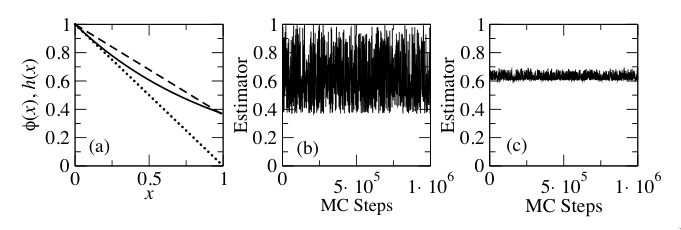
\includegraphics[width=\textwidth]{importance-sampling}
			\caption{The integrand and two possible importance functions}
			\label{fig:importance-sampling-example}
		\end{figure}

\section{Markov chains}

$$\tilde{I}_M = \frac{1}{M}\sum\limits_{i=1}^M\phi(x_i)$$

The vectors $x_1, x_2, \dots, x_M$ can be generated sequentially in a Markov chain: a rule to generate $x_{i+1}$ given $x_i$ is given.
$R(x|y)$ is the probability to obtain $x$ given $y$.
If there are two micro states it is the probability to move to a microstate $x$ from a microstate $y$.
Detailed balance condition:

$$R(x|y)f(y) = R(y|x)f(x)$$

\begin{itemize}
	\item Microscopic reversibility.
	\item Unbiased sampling of phase space.
	\item Sufficient but not strictly necessary condition to ensure proper sampling of phase space.
\end{itemize}

	\subsection{Rejection methods}
	$T(x|y)$ is a rule to generate a trial move or proposed move from $y$ to $x$.
	Normalization:

	$$\int dxT(x|y) = 1$$

	$A(x|y)$ is the probability to accept the move from $y$ to $x$:

	$$R(x|y) = A(x|y)T(x|y)$$

	By applying the detailed balance condition:

	$$A(x|y)T(x|y)f(y) = A(y|x)T(y|x)f(x)$$

	The acceptance probabilities are related.

	$$A(x|y) = \frac{T(y|x)f(x)}{T(x|y)f(y)}A(y|x) = r(x|y)A(y|x)$$

	If $A(x|y) = 1$ the move $y\rightarrow x$ is favoured $\Rightarrow A(y|x)< 1 \Rightarrow r(x|y)>1$.
	If $A(x|y) < 1$, $y\rightarrow x$ is not entirely favoured $\Rightarrow A(y|x) = 1\Rightarrow r(x|y) < 1$.

	$$A(x|y) = \min[1, r(x|y)]$$

	\subsection{Metropolis algorithm}
	The trial distribution $T(x_{k+1}|x_k)$ is used to propose a move $x_k\rightarrow x_{k+1}$:

	$$r(x_{k+1}|x_k) = \frac{T(x_k|x_{k+1})f(x_{k+1})}{T(x_{k+1}|x_k)f(x_k)}$$

	If $f(x_{k+1}|x_k)>1$ accept the move, otherwise accept the move with probability given by $r(x_{k+1}|x_k)$: extract a random number $\xi\in[0,1]$.
	If $\xi< r(x_{k+1}|x_k)$ accept the move.
	Associated probability for each point $x_1, \dots, x_n$: $\pi_1(x), \dots, \pi_n(x)$.

	$$\lim\limits_{n\rightarrow\infty}\pi_n(x) = f(x)$$

	Proof by recursive relation: $\pi_{n+1}(x)$ receives contributions from accepted moves starting at $y$ and ending in $x$ and from attempted moves to $y$ that are rejected:

	$$\pi_{n+1}(x) = \int A(x|y)T(x|y)\pi_n(y)dy + \pi_n(x)\int[1-A(y|x)]T(y|x)dy$$

	If $\pi_n(x) = f(x)$:

	$$\pi_{n+1} = \int A(x|y)T(x|y)f(y)dy + f(x)\int[1-A(y|x)]T(y|x)dy$$

	Detailed balance condition: $A(x|y)T(x|y)f(y) = A(y|x)T(y|x)f(x)$:

	$$\pi_{n+1}(x) = f(x)\int T(y|x)dy = f(x)$$

		\subsubsection{Summary}

		$$r(x|y) = \frac{T(y|x)f(x)}{T(x|y)f(y)}$$

		For a uniform choice of $T(x|y)$:

		$$r(x|y) = \frac{f(x)}{f(y)}\Rightarrow A(x|y) = \min\biggl[1, \frac{f(x)}{f(y)}\biggr]$$

	\subsection{Canonical distribution}

	$$Q(N, V, T) = \frac{1}{N!\lambda^{3N}}\int d\vec{r}_1\cdots d\vec{r}_Ne^{-\beta U(\vec{r}_1, \dots, \vec{r}_N)}$$

	$$A(r'|r) = \min\bigl[1, e^{-\beta(U(r')-U(r))}\bigr]$$

	$\Delta U < )$ accept the move.
	$\Delta U > 0$ accept the move with probability $e^{-\beta\Delta U}$.
	A Monte Carlo pass is equivalent to $N$ trial moves: particles must be chosen randomly.
	In one Monte Carlo pass each particle on average has seen one attempt.
	It is not necessary to recompute $U(r')$ in full at each move.

	$$\begin{cases}x'_i = x_i+\frac{1}{\sqrt{3}}(\xi_x-0.5)\Delta\\y'_i = y_i+\frac{1}{\sqrt{3}}(\xi_y-0.5)\Delta\\z'_i = z_i+\frac{1}{\sqrt{3}}(\xi_z-0.5)\Delta\end{cases}$$

	$\Delta$ must be chosen.

\section{Molecular dynamics and Monte Carlo methods}
In molecular dynamics:

\begin{multicols}{2}
	\begin{itemize}
		\item All particles move at once $\Delta t$.
		\item Information on dynamics.
		\item Parallel architectures.
	\end{itemize}
\end{multicols}

In Monte Carlo:

\begin{multicols}{2}
	\begin{itemize}
		\item There is no limit on the range of moves.
		\item Natural thermostats and barostats.
		\item Flexibility.
		\item Egodicity.
	\end{itemize}
\end{multicols}

	\subsection{Isothermal-isobaric ensemble}

	$$\delta(N, P, T) = \frac{1}{V_0} \int dVe^{-\beta PV}Q(N, V, T) = \frac{1}{V_0}\frac{1}{N!\lambda^{3N}}\int_0^{\infty}dVe^{-\beta PV}\int_Vd\vec{r}_1\cdots d\vec{r}_Ne^{-\beta U(\vec{r}_1, \dots, \vec{r}_N)}$$

	Previous scheme and trial moves on volume: $V' = V + (\xi_V-0.5)\delta$.
	Volume changes imply scaling of particle coordinates: $r'_i = \biggl(\frac{V'}{V}\biggr)^{\frac{1}{3}}r_i$.

	$$\Delta(N, P, T) = \frac{1}{V_0}\frac{1}{N!\lambda^{3N}}\int_0^{\infty}dVV^Ne^{-\beta PV}\int_Vd\vec{s}_1\cdots d\vec{s}_Ne^{-\beta U(V^{\frac{1}{3}}\vec{s}_1,\dots, V^{\frac{1}{3}}\vec{s}_N)}$$

	$$A(V'|V) = \min\bigl[1, e^{-\beta P(V'-V)e^{N\ln \frac{V'}{V}}e^{-\beta(U(r')-U(r))}}\bigr]$$

	$\delta$ should be small to accept the move.
	This is computational demanding, it less frequent with higher acceptance.

	\subsection{Gran canonical ensemble}

	$$\mathcal{E}(\mu, V, T) = \sum\limits_{N=0}^{\infty}e^{\beta\mu N}Q(N, V, T) = \sum\limits_{N+0}^{\infty}e^{\beta\mu N}\frac{1}{N!\lambda^{3N}}\int d\vec{r}_1\cdots d\vec{r}_Ne^{-\beta U(\vec{r}_1, \dots, \vec{r}_N)}$$

	This is the previous scheme with trial moves with particle insertion and particle deletion.
	Particle insertion:

	$$A(N+1|N) = \min\biggl[1, \frac{V}{\lambda^3(N+1)}e^{\beta\mu}e^{-\beta(U(r')-U(r))}\biggr]$$

	Particle deletion:

	$$A(N-1|N) = \min\biggl[1, \frac{\lambda^3V}{V}e^{-\beta\mu}e^{-\beta(U(r')-U(r))}\biggr]$$

	This is not so expensive: $U(r')$ requires only the change in energy due to one particle.

	\subsection{Hybrid Monte Carlo}
	Molecular dynamics is used as an engine to generate Monte Carlo moves:

	$$A(r', p' | r, p) = \min\{1, e^{-\beta[\mathcal{H}(r', p')-\mathcal{H}(r, p)]}\} = \min\bigl[1,e^{-\beta\Delta\mathcal{H}}\bigr]$$

	Symplectic time-reversible algorithm:

	$$T(r', p'|r, p) = T(r, -p|r', -p')$$

	One move is quite expensive, so it is better to have a higher acceptance rate between $40$ and $70\%$.
	In the case of a rejected move $p$ is resampled.
	If the integrator is time-reversible the detailed balance holds.

		\subsubsection{Detailed balance}
	Detailed balance condition:

		$$\int d^Npd^Np' T(r',p'|r,p)A(r',p'|r,p)f(r,p) = \int d^Npd^Np'T(r, p|r',p;)A(r,p|r',p')f(r',p')$$

		$$A(r',p'|r,p)f(r,p) = \frac{1}{Q_N(V, T)}\min\bigl[1, e^{-\beta(\mathcal{H}(r', p')-\mathcal{H}(r,p))}\bigr]e^{-\beta\mathcal{H}(r, p)}$$

		$$A(r',p'|r,p)f(r,p) = \frac{1}{Q_N(V, T)}\min\bigl[e^{-\beta\mathcal{H}(r, p)}, e^{-\beta\mathcal{H}(r', p')}\bigr]$$

		Similarly:

		$$A(r,p|r',p')f(r,'p') = \frac{1}{Q_N(V, T)}\min\bigl[e^{-\beta\mathcal{H}(r', p')}, e^{-\beta\mathcal{H}(r, p)}\bigr]$$

		Therefore: $A(r', p'|r, p)f(r, p) = A(r, p|r', p')f(r',p')$

		\subsubsection{Sympectic time-reversibility}
		Symplectic time-reversible algorithm:

		$$T(r', p'|r, p) = T(r, -p|r', -p')$$

		$$\int d^Npd^Np'T(r',p'|r, p)A(r', p'|r, p)f(r,p) = \int d^Npd^Np'T(r, -p|r', -p')A(r, p|r', p')f(r', p')$$

		Performing a change of variables: $p, p'\rightarrow -p, -p'$:

		$$\int d^Npd^Np'T(r',p'|r, p)A(r', p'|r, p)f(r,p) = \int d^Npd^Np'T(r,p|r', p')A(r, p|r', p')f(r',p')$$
